% Este documento se realizó con el propósito de proporcionale a los estudiantes
del CIDETEC un machote en latex de la tesis. Espero que les sirva de ayuda.
% Atte: Dr. Miguel Gabriel Villarreal Cervantes.
%*****************************************************************************
%*****************************************************************************
% Capítulo I
\chapter{Introducción \label{cap1}}

La computadora al igual que cualquier otra máquina fue diseñada para facilitar
la vida de las personas, ya sea acelerando o facilitando el trabajo realizado.
Actualmente hay tareas que se realizan en la computadora y se hacen de forma
mecanizada ya que no hay variantes en estas. 

Por mencionar algunas de las herramientas existentes  para la automatización
este tipo de tareas se tienen las siguientes:

Macros: son un conjunto de instrucciones que el fabricante del software ha
colocado para agilizar manejo de este; sin embargo, el usuario tiene  que
aprender cómo utilizarlas, por ejemplo, una combinación de teclas. También
existen opciones para crear macros personalizadas, ya sea por una opción que
da el fabricante o con software de terceros…

El capítulo \ref{cap1} 

En \cite{RolandSiegwart+IllanNourbakhsh},


Por lo tanto en este trabajo de investigación se propone, como un problema ....

\section{Estado del arte}
En esta sección se mostraran los trabajos relacionados o similares al proyecto
 propuesto y una breve descripción de estos. En la investigación realizada se 
 han encontrado trabajos cuyo objetivo es obtener que un robot mecánico o
 virtual realice tareas de manera similar a como las haría un humano. 

Empezando por un trabajo desarrollado por la Universidad de Tsukuba en
 Japón\cite{Nakano2006}, tiene por objetivo el crear un oponente virtual
 al nivel de un oponente humano que represente un reto para el jugador. Para
 lograr esto se crearon perfiles con el comportamiento de los jugadores y
 posteriormente se reproducen en otra partida.

En el trabajo desarrollado en la Universidad Tecnológica de Lanzhou en China
 \cite{Zhang2017},hacen un análisis del comportamiento del soldador experto
 humano utilizando un sistema de inferencia neurodifuso adaptativo (ANFIS,
 por sus siglas en ingles) para su automatización, considerando las variables
 de los materiales usados y caracterizando la tarea del soldador humano. 

En el ambiente artístico \cite{Nishiguchi2017}, el trabajo desarrollado en
 Japón por la Universidad de artes de Tokyo y la Universidad de Osaka, cuyo
 objetivo era brindar un comportamiento natural humano a un Robot Humanoide.
 Para cumplir esto utilizaron el conocimiento del director de escena Hirata,
 que dada la precisión en sus instrucciones a los actores, facilita la
 traducción de esas órdenes a las reglas para el robot humanoide, además,
 desarrollaron una interfaz de usuario para que el manejo del robot sea más
 sencillo, ayudando a los principiantes, ya que proporcionan menos datos se
 puede obtener buenos resultados.

El trabajo desarrollado por la Universidad de Plymouth, Universidad de Lincoln
 ambas en el Reino Unido y la Universidad de Gante en Bélgica\cite{Senft2016},
 realiza la comparativa de su método SPARC (Supervised Progressively Autonomous
 Robot Competencies) con el IRL (Interactive Reinforcement Learning), estos dos
 métodos se basan en el aprendizaje automático de un robot, haciendo que un
 humano con conocimiento del tema de la aprobación de la actividad que está
 realizando o que va a realizar el robot.



\section{Justificación}
A nivel mundial, la discapacidad va en aumento dado que la población está
 envejeciendo y son pocos los programas privados y gubernamentales que apoyan a
 este grupo de personas. Con referencia a los datos obtenidos Censo de Población
 y Vivienda de 2010 era poco más del 5\% de la Población de México la que
 presentaba algún tipo de discapacidad, pero se puede apreciar que esta cifra va
 en aumento ya que en la Encuesta Nacional de Ingresos y Gasto de los Hogares
 (ENIGH) de 2012 fue el 6.6\% el porcentaje de la población la que tenía alguna
 discapacidad.
 
 
La Organización Mundial de la Salud (OMS) y el Banco Mundial proponen una
 estrategia de colaboración entre el sector privado y gubernamental para
 rehabilitar e incorporar a la sociedad a las personas discapacitadas y así
 poder aprovechar el potencial de toda esta gente.
 
 
Algunas de estas propuestas tienen por objetivo proporcionar accesibilidad en
 los servicios convencionales, por ejemplo transporte y educación, así como
 adiestrar a los servidores públicos, para que las personas sean tratadas con
 los cuidados necesarios.
 
 
Como un apoyo a las personas que por su discapacidad presentan dificultad para
 interactuar de manera ágil y precisa con las computadoras de escritorio, se
 plantea desarrollar un sistema de reconocimiento de patrones con la capacidad
 reproducir las acciones que tengan mayor incidencia de uso.

\section{Planteamiento del problema}
Con base en lo mencionado previamente, se puede apreciar que la población de
 Personas con Movilidad Reducida(PRM) va en aumento en México y con el uso de
 la computadora como algo imprescindible en la actualidad sobre todo en el
 sector laboral 2, la discapacidad de estas personas puede representar un
 obstáculo en su desarrollo laboral.



\section{Objetivo general} 
Diseñar y desarrollar un software que defina a partir de un periodo de tiempo
 determinado el conjunto de acciones con mayor incidencia de uso por un usuario
 realizadas en una computadora por un usuario, para su uso posterior.

\section{Objetivos específicos}
\begin{itemize}
  \item Desarrollar del sistema para la captura de acciones, tanto del  ratón
  como del teclado.
  \item Obtener una muestra de las acciones realizadas con el teclado y el 
  ratón por un usuario en una computadora.
  \item Diseñar y desarrollar el algoritmo para la determinación de tareas
  repetitivas.
\end{itemize}


\section{Metodología}
Con el propósito de desarrollar y lograr los objetivos propuestos en el presente trabajo de investigación, se plantearon siguientes metas:
\section*{Metas}
\begin{itemize}
  \item[I] Investigación de sistemas similares.
  \item[II] Recopilación de resultados de sistemas similares.
  \item[III] Desarrollo del sistema  de captura de datos.
  \item[IV] Obtención de los datos de ejemplo.
  \item[V] Desarrollo del Sistema de procesamiento de datos.
  \item[VI] Realizar pruebas del sistema.
  \item[VII] Realizar comparativa de los resultados.
\end{itemize}





\section{Cronograma de actividades}

\begin{figure}[h]
\centering
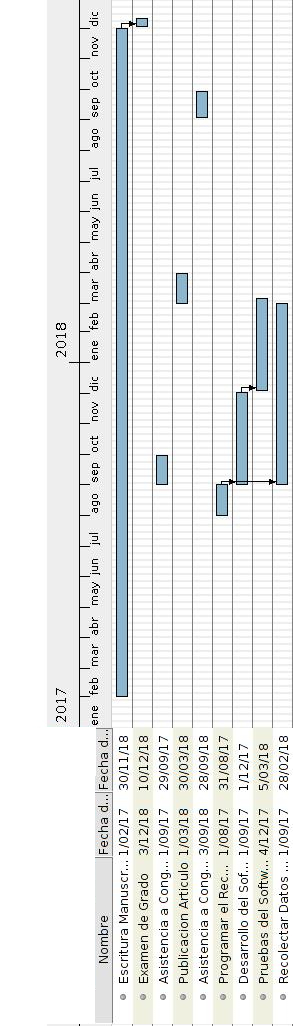
\includegraphics[width=0.3\columnwidth]{./CapituloI/Imagenes/Cronograma.jpg}
\end{figure}


